\documentclass{beamer}

\usepackage{style}
\usepackage{beamer}

\usepackage[backend=bibtex8]{biblatex}
\addbibresource{src_2025.bib}

\usepackage{subcaption}

\graphicspath{ {./figures/} }

\title{Identifying Models of Fluid Flow with Nudging and Gradient-based Optimization}
\author{Nathan Schill}
\institute{Brigham Young University}
\date{March 8, 2025}

\AtBeginSection[]
{
  \begin{frame}
    \frametitle{Table of Contents}
    \tableofcontents[currentsection]
  \end{frame}
}

\renewcommand{\b}{\boldsymbol}
\newcommand{\bu}{\boldsymbol u}
\newcommand{\bv}{\boldsymbol v}
\newcommand{\bw}{\boldsymbol w}

\newcommand{\ol}{\overline}

\newcommand\blfootnote[1]{%
  \begingroup
  \renewcommand\thefootnote{}\footnote{#1}%
  \addtocounter{footnote}{-1}%
  \endgroup
}

\begin{document}

\frame{\titlepage}

\section{Goal}

\begin{frame}
  \frametitle{Two-dimensional turbulence \cite{guan_online_2024}}

  \begin{align*}
    \omega & \quad \text{vorticity} \\
    \psi & \quad \text{streamfunction}
  \end{align*}
  ``True'' system state
  \begin{equation}
    \begin{gathered}
      \nabla^2 \psi = - \omega \\
      \frac{\partial \omega}{\partial t} + \mathcal N(\omega, \psi)
      = \frac1{Re} \nabla^2 \omega - f - r \omega
      + \beta \frac{\partial \psi}{\partial x}
    \end{gathered}
  \end{equation}

  \begin{figure}
    \centering
    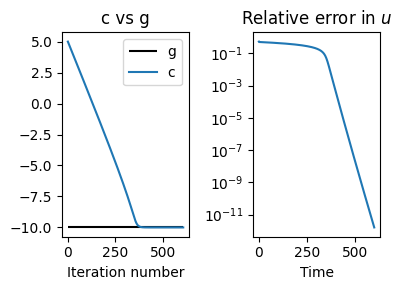
\includegraphics[width=3cm, height=3cm, keepaspectratio]{placeholder.png}
    % One of Karan's figures
  \end{figure}
\end{frame}

\begin{frame}
  \frametitle{Goal}
  Wish: simulate every atom continuously
  % \pause

  Reality: simulate on a coarse spatial and temporal grid
  \newline
  % \pause

  Apply low-pass filter to true system equation to simulate coarse resolution
  of simulation
  \begin{equation}
    \begin{gathered}
      \nabla^2 \ol \psi = - \ol \omega \\
      \frac{\partial \ol \omega}{\partial t} + \mathcal N(\ol \omega, \ol \psi)
      = \frac1{Re} \nabla^2 \ol \omega - \ol f - r \ol \omega
      + \beta \frac{\partial \ol \psi}{\partial x}
      - \underbrace{
        \bbrack*{\ol{\mathcal N(\omega, \psi)}
        - \mathcal N(\ol \omega, \ol \psi)}
        % }_{\text{subgrid-scale (\textcolor{red}{SGS}) term}}
      }_{\text{subgrid-scale (} \textcolor{red}{\text{SGS}} \text{) term}}
    \end{gathered}
  \end{equation}

  \begin{figure}
    \centering
    \begin{subfigure}{0.45\textwidth}
      \centering
      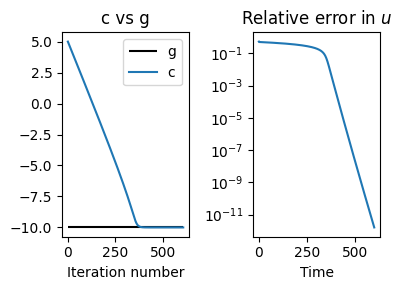
\includegraphics[width=3cm, height=3cm, keepaspectratio]{placeholder.png}
      % One of Karan's figures
    \end{subfigure}
    \begin{subfigure}{0.45\textwidth}
      \centering
      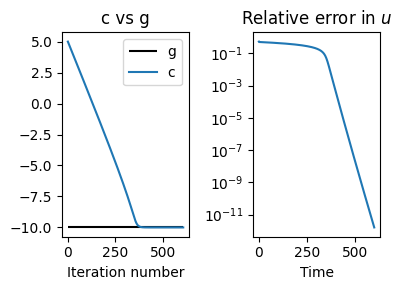
\includegraphics[width=3cm, height=3cm, keepaspectratio]{placeholder.png}
      % One of Karan's figures
    \end{subfigure}
  \end{figure}
\end{frame}

\begin{frame}
  \frametitle{Question}

  \textcolor{gray}{
    \begin{equation*}
      \begin{gathered}
        \nabla^2 \ol \psi = - \ol \omega \\
        \frac{\partial \ol \omega}{\partial t} + \mathcal N(\ol \omega, \ol \psi)
        = \frac1{Re} \nabla^2 \ol \omega - \ol f - r \ol \omega
        + \beta \frac{\partial \ol \psi}{\partial x}
        - \underbrace{
          \bbrack*{\ol{\mathcal N(\omega, \psi)}
          - \mathcal N(\ol \omega, \ol \psi)}
          % }_{\text{subgrid-scale (\textcolor{red}{SGS}) term}}
        }_{\text{subgrid-scale (} \textcolor{red}{\text{SGS}} \text{) term}}
      \end{gathered}
    \end{equation*}
  }

  \begin{block}{Question}
    How do we \textit{estimate} an optimal SGS term?
  \end{block}
\end{frame}

\section{More on the parameter estimation framework}

\begin{frame}
  \frametitle{True system}
  ``True'' system state $\bu: \Omega \times [a, b] \rightarrow \R^n$
  \begin{equation*}
    \frac{\partial \bu}{\partial t} + F(\bu, \gamma) = 0
  \end{equation*}
  \begin{align*}
    &\gamma \in \R^p &&\text{true parameters} \\
    &F: \R^n \times \R^p \rightarrow \R^n &&\text{function defining true
    differential equation} \\
    &\Omega \subseteq \R^d &&\text{spatial domain (if PDE)} \\
    &[a, b] \subseteq \R &&\text{time domain (possibly infinite)}
  \end{align*}
\end{frame}

\begin{frame}
  \frametitle{Estimated system}
  \textcolor{gray}{
    ``True'' system state $\bu: \Omega \times [a, b] \rightarrow \R^n$
    \begin{equation*}
      \frac{\partial \bu}{\partial t} + F(\bu, \gamma) = 0
    \end{equation*}
  }

  \vskip 0.5em

  Estimated, ``nudged'' system state $\bv: \Omega \times [a, b] \rightarrow \R^n$
  \begin{equation*}
    \frac{\partial \bv}{\partial t} + G(\bv, c) = \mu I_h(\bu - \bv)
  \end{equation*}
  \begin{align*}
    &G: \R^n \times \R^{\textcolor{red}q} \rightarrow \R^n &&\text{function
    defining estimated differential equation} \\
    &I_h: \R^n \rightarrow \R^n &&\text{(linear) observation operator} \\
    &\mu \in \R_{\ge 0} &&\text{nudging coefficient} \\
    &c \in \R^{\textcolor{red}q} &&\text{estimated parameters}
  \end{align*}
\end{frame}

\begin{frame}
  \frametitle{Define error and derivative}
  Define an error between the true and estimated states; for example,
  \begin{equation*}
    E(c) \coloneq \frac12 \norm*{I_h(\bv - \bu)}^2 \bigg \lvert_{t=t_0}
    = \frac12 \innerproduct*{I_h(\bv - \bu), I_h(\bv - \bu)} \bigg \lvert_{t=t_0}
  \end{equation*}
  % \pause

  Differentiate with respect to the $i$th parameter, $c_i$:
  \begin{equation*}
    \frac{\partial}{\partial c_i} E(c) = \innerproduct*{I_h(\bv - \bu),
    I_h \bw_i} \bigg \lvert_{t=t_0}
  \end{equation*}
  where $\bw_i \coloneq \frac{\partial \bv}{\partial c_i}$ is the $i$th
  \textit{sensitivity}.
  % \pause

  If we can compute $\bw_i$, we can perform gradient descent to minimize error.
\end{frame}

\begin{frame}
  \frametitle{Estimate $\bw_i$}
  Some boring differentiation
  \begin{alignat*}{4}
    \frac{\partial}{\partial c_i} \left(\frac{\partial \bv}{\partial t}\right.
      &+ G(\bv, c)
    &&&&= \mu I_h(\bu - \bv)\bigg) \\
    \dot \bw_i
    &+ \frac{\partial G}{\partial \bv} \bw_i
    &&+ G_{c_i}(\bv, c)
    &&= \mu I_h \bw_i
  \end{alignat*}
  % \pause

  Estimate $\bw_i$ asymptotically as $\mu \rightarrow \infty$ by assuming
  \begin{equation*}
    \bw_i = \bw_i^{0} + \frac1\mu \bw_i^{1} + \frac1{\mu^2} \bw_i^{2} + \cdots
  \end{equation*}
  and equating like terms in $\mu$.
  % \pause

  \vskip 0.5em

  A scaling of time $\tau = \mu t$ and an application of Watson's Lemma yield
  \begin{equation*}
    I_h \bw_i(t) \sim - \frac1\mu I_h G_{c_i}(\bv(t), c)
  \end{equation*}
\end{frame}

\section{Steps}

\subsection{Write code supporting framework}

\begin{frame}
  \frametitle{Framework code}
  Construct classes to easily implement
  \begin{itemize}[label=\checkmark]
    \item<1-> systems of differential equations
    \item<2-> differential equation solvers
    \item<3-> optimization of parameters
  \end{itemize}
  \pause
  \pause
  \pause

  \begin{figure}
    \centering
    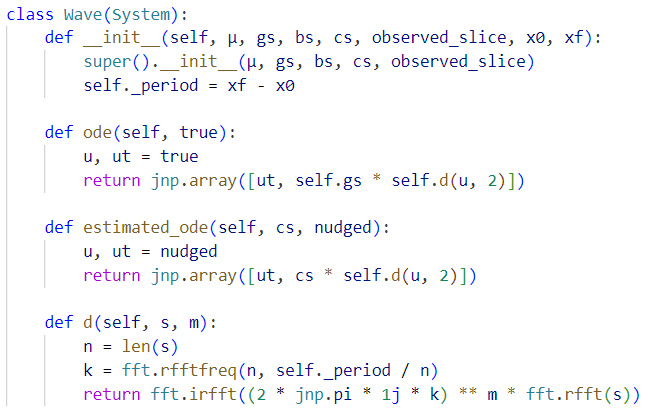
\includegraphics[height=2in, keepaspectratio]{wave_1d_code.png}
  \end{figure}
\end{frame}

\subsection{Test on ordinary differential equations}

\subsection{Test on partial differential equations}

\begin{frame}
  \frametitle{Test on PDEs: one-dimensional wave equation}
  \begin{figure}
    \centering
    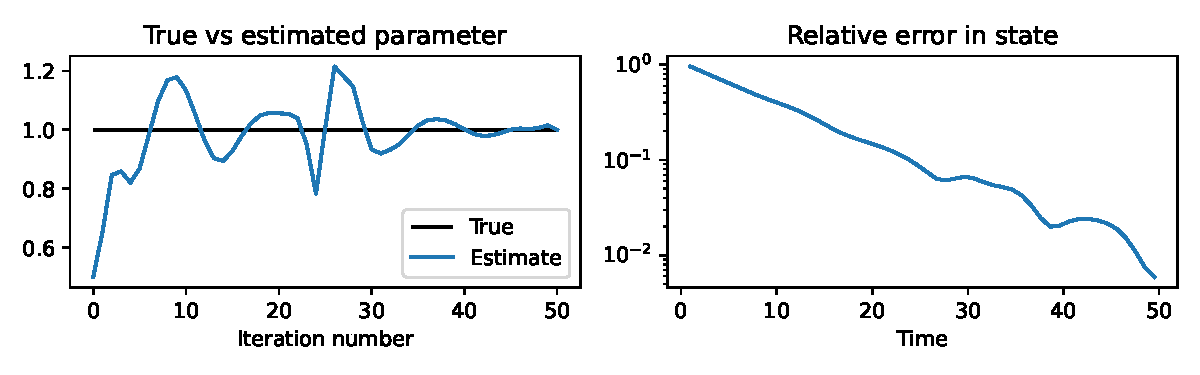
\includegraphics[width=0.9\textwidth, keepaspectratio]{wave_1d_params.pdf}
  \end{figure}
  \vskip -1em
  \begin{figure}
    \centering
    \begin{subfigure}{0.42\textwidth}
      \centering
      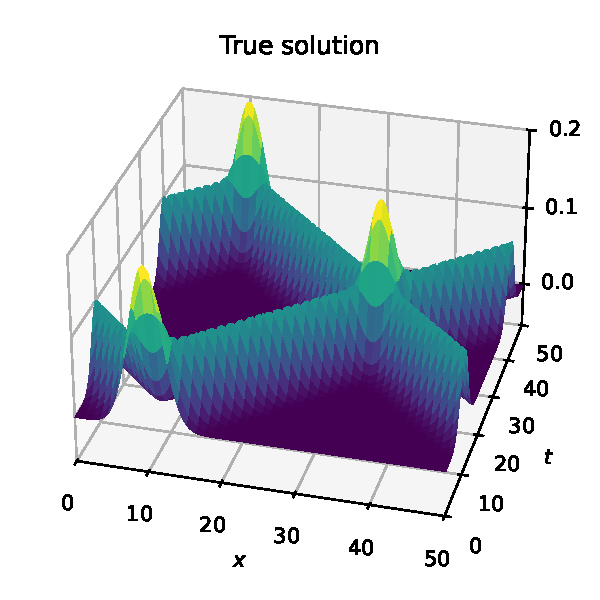
\includegraphics[width=\textwidth, keepaspectratio]{wave_1d_true.pdf}
    \end{subfigure}
    \begin{subfigure}{0.42\textwidth}
      \centering
      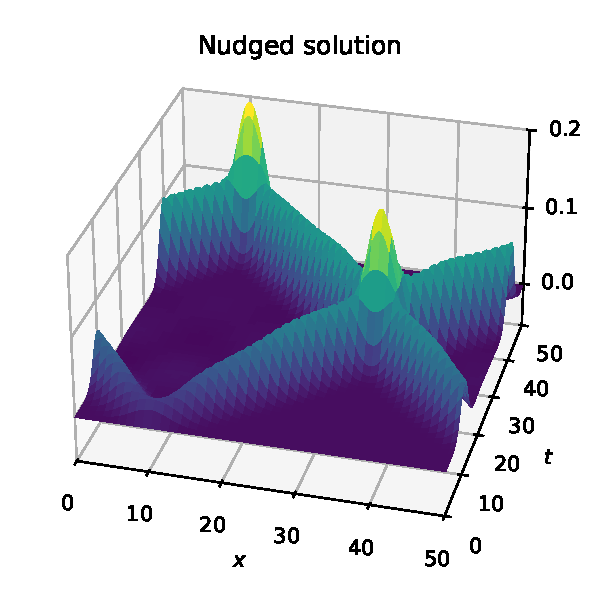
\includegraphics[width=\textwidth, keepaspectratio]{wave_1d_nudged.pdf}
    \end{subfigure}
  \end{figure}
\end{frame}

\section{Current and future work}

\begin{frame}
  \frametitle{Current and future work}
  \begin{itemize}[label=+]
    \item<1-> Apply method to Kuramoto--Sivashinsky
      equation\blfootnote{Image:
      \text{en.wikipedia.org/wiki/Kuramoto--Sivashinsky\_equation}}
      \begin{equation*}
        u_t + u_{xx} + u_{xxxx} + u u_x = 0
      \end{equation*}
    \item<2-> Clarify application of asymptotics to PDEs
    \item<3-> Add regularization on parameter magnitudes
    \item<4-> Experiment with alternative definitions of error $E(c)$
    \item<5-> Apply method to two-dimensional turbulence
  \end{itemize}
  \begin{figure}
    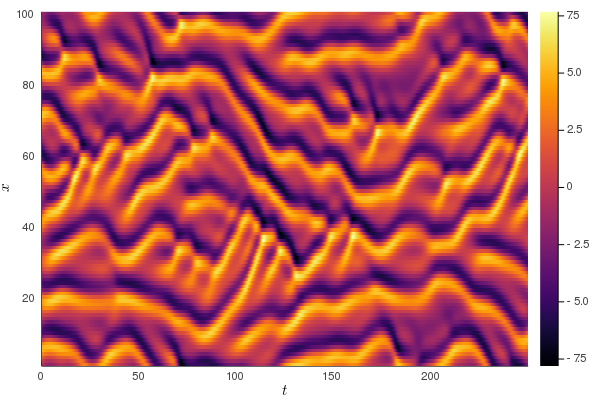
\includegraphics[height=1.5in, keepaspectratio]{kse.png}
  \end{figure}
\end{frame}

\begin{frame}
  \frametitle{References}
  \nocite{*}
  % \printbibliography
\end{frame}

\end{document}
